% 서울대학교 학사 학위논문 - SE-gated Cascade를 통한 LLM 환각 탐지
\RequirePackage{fix-cm}
\documentclass[oneside,ko,under]{snuthesis}

%%%%%%%%%%%%%%%%%%%%%%%%%%%%%%%%%%%%%%%% 
%% 목차 양식
\usepackage[titles]{tocloft}
\makeatletter
\if@snu@ko
	\renewcommand\cftchappresnum{제\ }
	\renewcommand\cftchapaftersnum{\ 장\quad}
	\renewcommand\cftfigpresnum{그림\ }
	\renewcommand\cftfigaftersnum{\quad}
	\renewcommand\cfttabpresnum{표\ }
	\renewcommand\cfttabaftersnum{\quad}
\else
	\renewcommand\cftchappresnum{Chapter~}
	\renewcommand\cftfigpresnum{Figure~}
	\renewcommand\cfttabpresnum{Table~}
\fi
\makeatother
\newlength{\mytmplen}
\settowidth{\mytmplen}{\bfseries\cftchappresnum\cftchapaftersnum}
\addtolength{\cftchapnumwidth}{\mytmplen}
\settowidth{\mytmplen}{\bfseries\cftfigpresnum\cftfigaftersnum}
\addtolength{\cftfignumwidth}{\mytmplen}
\settowidth{\mytmplen}{\bfseries\cfttabpresnum\cfttabaftersnum}
\addtolength{\cfttabnumwidth}{\mytmplen}
%%%%%%%%%%%%%%%%%%%%%%%%%%%%%%%%%%%%%%%%

%%%%%%%%%%%%%%%%%%%%%%%%%%%%%%%%%%%%%%%%
%% 패키지 로드
\usepackage{graphicx}
\usepackage{amsmath}
\usepackage{amssymb}
\usepackage{booktabs}
\usepackage{multirow}
\usepackage{algorithm}
\usepackage{algorithmic}
\usepackage{url}
\usepackage{kotex}
\usepackage{fontspec}
\usepackage{listings}
\usepackage{xcolor}
\usepackage{tikz}
\usetikzlibrary{shapes,arrows,positioning,calc,backgrounds,shapes.geometric,arrows.meta,fit}
\usepackage{pgfplots}
\pgfplotsset{compat=1.18}

% TikZ 다이어그램 정의 파일
% TikZ 다이어그램 - 학술 논문 스타일
% 색상 팔레트 정의
\definecolor{primaryblue}{RGB}{31,119,180}
\definecolor{secondaryorange}{RGB}{255,127,14}
\definecolor{accentgreen}{RGB}{44,160,44}
\definecolor{accentpurple}{RGB}{148,103,189}
\definecolor{neutralgray}{RGB}{127,127,127}
\definecolor{lightgray}{RGB}{200,200,200}
\definecolor{hallred}{RGB}{214,39,40}
\definecolor{normgreen}{RGB}{44,160,44}

%=============================================================================
% Figure 1: SE-Gated Cascade 개념도 (깔끔한 플로우차트)
%=============================================================================
\newcommand{\cascadediagram}{
\begin{tikzpicture}[
    node distance=1.5cm,
    >={Stealth[length=2.5mm]},
    box/.style={
        rectangle, draw=black!70, line width=0.8pt,
        rounded corners=2pt, minimum width=3cm, minimum height=0.9cm,
        align=center, font=\small
    },
    inputbox/.style={box, fill=lightgray!30},
    processbox/.style={box, fill=primaryblue!15},
    energybox/.style={box, fill=secondaryorange!20},
    outputbox/.style={box, fill=accentgreen!20},
    decision/.style={
        diamond, draw=black!70, line width=0.8pt,
        aspect=2.5, minimum width=2cm, align=center, font=\small,
        fill=accentpurple!15
    },
    arrow/.style={->, line width=0.8pt, black!70},
    label/.style={font=\scriptsize, text=black!60}
]

% 상단: 입력 → 샘플링 → 클러스터링 (가로)
\node[inputbox] (input) {Input: 질문 $q$};
\node[processbox, right=2cm of input] (sample) {LLM 샘플링 ($K$=5)};
\node[processbox, right=2cm of sample] (cluster) {NLI 클러스터링};

% 중단: 메트릭 계산 (병렬)
\node[processbox, below left=1.5cm and 0.3cm of cluster] (se) {SE 계산};
\node[energybox, below right=1.5cm and 0.3cm of cluster] (energy) {Energy 계산};

% 하단: 분기 및 출력
\node[decision, below=2.5cm of cluster] (gate) {$|C|=1$?};
\node[outputbox, below=1.8cm of gate] (output) {환각 점수};

% 화살표
\draw[arrow] (input) -- (sample);
\draw[arrow] (sample) -- (cluster);
\draw[arrow] (cluster) -- (se);
\draw[arrow] (cluster) -- (energy);
\draw[arrow] (se) -- (gate);
\draw[arrow] (energy) -- (gate);
\draw[arrow] (gate) -- node[right, label] {Energy (Yes) / SE (No)} (output);

% 클러스터 수 표시
\node[font=\scriptsize, text=black!50, right=0.1cm of cluster] {$\rightarrow |C|$};

\end{tikzpicture}
}

%=============================================================================
% Figure 2: Zero-SE 현상 요약 (3-panel) - 완전 정렬 버전
%=============================================================================
\newcommand{\zerosefigure}{
\centering
\begin{tikzpicture}[font=\small]

% 모든 패널: y=0 ~ y=2.5 범위, 제목은 y=-0.5

% Panel A: 파이 차트 (하단을 y=0에 맞춤, 중심=radius)
\begin{scope}
    \def\radius{1.1}
    \def\centery{1.1}  % 중심 y = radius이면 하단이 y=0
    \fill[primaryblue!50] (0,\centery) circle (\radius);
    \fill[hallred!60] (0,\centery) -- ++(90:\radius) arc (90:21.6:\radius) -- cycle;
    
    \node[font=\scriptsize, white] at ($(0,\centery)+(55:0.7)$) {\textbf{19\%}};
    \node[font=\scriptsize, white] at ($(0,\centery)+(-70:0.6)$) {\textbf{81\%}};
    
    % 범례 (막대 차트 높이에 맞춤)
    \fill[hallred!60] (1.5,1.8) rectangle (1.75,2.0);
    \node[font=\tiny, anchor=west] at (1.8, 1.9) {Zero-SE};
    \fill[primaryblue!50] (1.5,1.4) rectangle (1.75,1.6);
    \node[font=\tiny, anchor=west] at (1.8, 1.5) {Non-Zero};
\end{scope}
\node[font=\scriptsize\bfseries] at (0,-0.5) {(a) Zero-SE 비율};
\node[font=\tiny, text=black!60] at (0,-0.85) {n=200};

% Panel B: 환각/정상 막대 (y=0 ~ 2.5)
\begin{scope}[xshift=5cm]
    \draw[->, black!70] (0,0) -- (0,2.6);
    \draw[->, black!70] (0,0) -- (2.5,0);
    
    \fill[hallred!60] (0.3,0) rectangle (0.95,2.15);
    \node[font=\scriptsize] at (0.625,2.3) {\textbf{28}};
    
    \fill[normgreen!60] (1.3,0) rectangle (1.95,0.77);
    \node[font=\scriptsize] at (1.625,0.92) {\textbf{10}};
    
    \node[font=\tiny] at (0.625,-0.2) {환각};
    \node[font=\tiny] at (1.625,-0.2) {정상};
    
    \node[font=\tiny, anchor=east] at (-0.05,0) {0};
    \node[font=\tiny, anchor=east] at (-0.05,2.15) {28};
\end{scope}
\node[font=\scriptsize\bfseries] at (6.1,-0.5) {(b) Zero-SE 구성};
\node[font=\tiny, text=black!60] at (6.1,-0.85) {환각률: 73.7\%};

% Panel C: Energy AUROC (y=0 ~ 2.5)
\begin{scope}[xshift=9.2cm]
    \draw[->, black!70] (0,0) -- (0,2.6);
    \draw[->, black!70] (0,0) -- (2,0);
    
    \draw[dashed, black!40, line width=0.5pt] (0,1.25) -- (1.7,1.25);
    \node[font=\tiny, text=black!40, anchor=west] at (1.4,1.35) {0.5};
    
    \fill[secondaryorange!70] (0.4,0) rectangle (1.2,1.84);
    \node[font=\scriptsize] at (0.8,2.0) {\textbf{0.736}};
    
    \node[font=\tiny] at (0.8,-0.2) {Energy};
    
    \node[font=\tiny, anchor=east] at (-0.05,0) {0};
    \node[font=\tiny, anchor=east] at (-0.05,2.5) {1.0};
\end{scope}
\node[font=\scriptsize\bfseries] at (10,-0.5) {(c) Zero-SE 탐지};

\end{tikzpicture}
}

%=============================================================================
% Figure 3: SE vs Energy Crossover (Grouped Bar)
%=============================================================================
\newcommand{\crossoverfigure}{
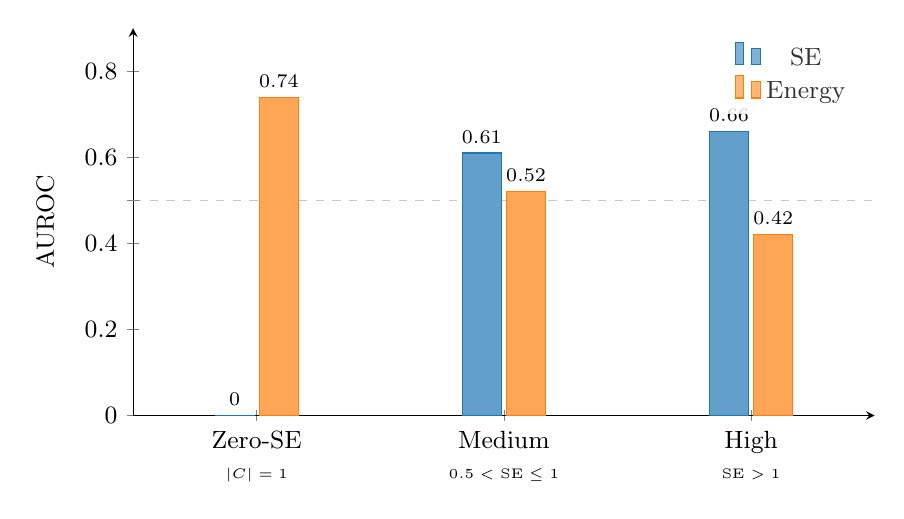
\begin{tikzpicture}
\begin{axis}[
    ybar,
    width=11cm, height=6.5cm,
    bar width=14pt,
    ylabel={AUROC},
    ylabel style={font=\small},
    ymin=0, ymax=0.9,
    xtick={1,2,3},
    xticklabels={Zero-SE\\{\tiny $|C|=1$}, Medium\\{\tiny $0.5<\text{SE}\leq1$}, High\\{\tiny $\text{SE}>1$}},
    xticklabel style={align=center, font=\small},
    tick label style={font=\small},
    legend style={
        at={(0.98,0.98)}, anchor=north east, 
        font=\small, 
        draw=none, fill=white, fill opacity=0.8,
        legend columns=1
    },
    nodes near coords,
    nodes near coords style={font=\scriptsize, /pgf/number format/.cd, fixed, precision=2},
    axis lines=left,
    enlarge x limits=0.25,
    extra y ticks={0.5},
    extra y tick style={grid=major, grid style={dashed, lightgray, line width=0.5pt}},
    extra y tick labels={},
    ymajorgrids=false,
]
\addplot[fill=primaryblue!70, draw=primaryblue] coordinates {(1,0.001) (2,0.61) (3,0.66)};
\addplot[fill=secondaryorange!70, draw=secondaryorange] coordinates {(1,0.74) (2,0.52) (3,0.42)};
\legend{SE, Energy}
\end{axis}

% 주석
% (요청 반영) 우세 방향 화살표/주석 제거

\end{tikzpicture}
}

%=============================================================================
% Figure 4: 상보성 분석 - 단순 막대 그래프
%=============================================================================
\newcommand{\complementarityfigure}{
\centering
\begin{tikzpicture}[font=\small]
% 축
\draw[->] (0,0) -- (0,5.5);
\draw[->] (0,0) -- (10,0);

% Y축 라벨 및 눈금
\node[font=\small, rotate=90, anchor=south] at (-0.6,2.75) {환각 샘플 수};
\foreach \y/\val in {0/0, 1.08/20, 2.16/40, 3.24/60, 4.32/80, 5.4/108} {
    \draw (-0.1,\y) -- (0.1,\y);
}
\node[font=\tiny, left] at (0,0) {0};
\node[font=\tiny, left] at (0,2.7) {50};
\node[font=\tiny, left] at (0,5.4) {108};

% 막대 1: SE만 (22)
\fill[primaryblue!70] (0.8,0) rectangle (2,1.1);
\node[font=\scriptsize] at (1.4,1.3) {22};
\node[font=\tiny, text=black!60] at (1.4,1.6) {(13.4\%)};
\node[font=\scriptsize, align=center] at (1.4,-0.4) {SE만\\탐지};

% 막대 2: Energy만 (22)
\fill[secondaryorange!70] (2.8,0) rectangle (4,1.1);
\node[font=\scriptsize] at (3.4,1.3) {22};
\node[font=\tiny, text=black!60] at (3.4,1.6) {(13.4\%)};
\node[font=\scriptsize, align=center] at (3.4,-0.4) {Energy만\\탐지};

% 막대 3: 둘 다 (12)
\fill[accentpurple!60] (4.8,0) rectangle (6,0.6);
\node[font=\scriptsize] at (5.4,0.8) {12};
\node[font=\tiny, text=black!60] at (5.4,1.1) {(7.3\%)};
\node[font=\scriptsize, align=center] at (5.4,-0.4) {둘 다\\탐지};

% 막대 4: 미탐지 (108)
\fill[neutralgray!50] (6.8,0) rectangle (8,5.4);
\node[font=\scriptsize] at (7.4,5.6) {108};
\node[font=\tiny, text=black!60] at (7.4,5.9) {(65.9\%)};
\node[font=\scriptsize, align=center] at (7.4,-0.4) {미탐지};

% 합집합 강조 박스
\draw[rounded corners=3pt, fill=accentgreen!15, draw=accentgreen!60, line width=1pt] 
    (0.5, 6.3) rectangle (5.5, 7.0);
\node[font=\small] at (3, 6.65) {합집합 탐지율: \textbf{34.1\%}};

% 제목
\node[font=\small\bfseries] at (4.5, 7.5) {상보성 분석 (n=164 환각)};

\end{tikzpicture}
}

%=============================================================================
% Figure 5: 전체 성능 비교 (Simple Bar)
%=============================================================================
\newcommand{\overallfigure}{
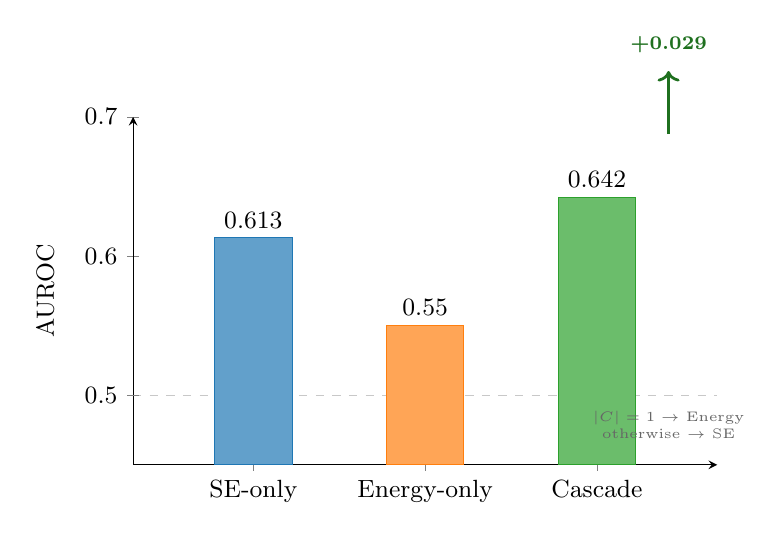
\begin{tikzpicture}
\begin{axis}[
    ybar,
    width=9cm, height=6cm,
    bar width=28pt,
    ylabel={AUROC},
    ylabel style={font=\small},
    ymin=0.45, ymax=0.70,
    xtick={1,2,3},
    xticklabels={SE-only, Energy-only, Cascade},
    xticklabel style={font=\small},
    tick label style={font=\small},
    nodes near coords,
    nodes near coords style={font=\small, /pgf/number format/.cd, fixed, precision=3},
    axis lines=left,
    enlarge x limits=0.35,
    extra y ticks={0.5},
    extra y tick style={grid=major, grid style={dashed, lightgray}},
    extra y tick labels={},
]
\addplot[fill=primaryblue!70, draw=primaryblue, bar shift=0pt] coordinates {(1,0.613)};
\addplot[fill=secondaryorange!70, draw=secondaryorange, bar shift=0pt] coordinates {(2,0.550)};
\addplot[fill=accentgreen!70, draw=accentgreen, bar shift=0pt] coordinates {(3,0.642)};
\end{axis}

% 개선 화살표
\draw[->, line width=1pt, accentgreen!70!black] (6.8, 4.2) -- (6.8, 5.0);
\node[font=\scriptsize, text=accentgreen!70!black, anchor=south] at (6.8, 5.1) {\textbf{+0.029}};

% Cascade 설명
\node[font=\tiny, text=black!60, align=center, anchor=north] at (6.8, 0.8) {$|C|=1 \rightarrow$ Energy\\otherwise $\rightarrow$ SE};

\end{tikzpicture}
}


\setmainfont{NanumSquare}
\setsansfont{NanumSquare}
% 모노스페이스 폰트는 시스템 기본 사용 (NanumSquare는 모노스페이스 아님)

% 코드 스타일
\lstset{
    basicstyle=\footnotesize\ttfamily,
    breaklines=true,
    frame=single,
    language=Python,
    keywordstyle=\color{blue},
    commentstyle=\color{gray},
    columns=flexible,
    showspaces=false,
    showstringspaces=false,
}
%%%%%%%%%%%%%%%%%%%%%%%%%%%%%%%%%%%%%%%%

\title{Semantic Entropy와 Semantic Energy의\\%
상보적 결합을 통한 LLM 환각 탐지:\\%
Zero-SE 문제 해결을 중심으로}

\schoolko{서울대학교}
\departmentko{자유전공학부}

\author{문정혁}
\author*{문~정~혁}

\studentnumber{2016-10749}

\advisor{김남수}
\advisor*{김~남~수}

\graddate{2026~년~2~월}
\approvaldate{2026~년~2~월~13일}

\begin{document}
\pagenumbering{Roman}
\makefrontcover
\makeapproval

\cleardoublepage
\pagenumbering{roman}

\keyword{대규모 언어모델, 환각 탐지, Semantic Entropy, Semantic Energy, Zero-SE 문제, SE-gated Cascade}
\begin{abstract}
대규모 언어모델(LLM)의 환각(hallucination) 문제는 실용적 적용에 있어 가장 심각한 장애물 중 하나이다. Farquhar 등이 Nature(2024)에서 제안한 Semantic Entropy(SE)는 LLM의 의미적 불확실성을 측정하는 대표적 방법이나, 모델이 일관되게 틀린 답변을 생성하는 Zero-SE 문제에서 한계를 보인다.

본 연구에서는 SE와 Semantic Energy의 상보적 특성을 분석하고, SE가 낮을 때 Energy로 대체하는 SE-gated cascade 방법을 제안한다. 핵심 통찰은 환각이 두 가지 유형---혼란(confusion)과 지어냄(confabulation)---으로 구분되며, SE는 전자를, Energy는 후자를 효과적으로 탐지한다는 것이다.

TruthfulQA 데이터셋 200개 샘플(K=5)에서의 실험 결과:
\begin{itemize}
    \item Zero-SE 영역이 전체의 19\%를 차지하며, 이 중 73.7\%가 환각
    \item Zero-SE 영역에서 Energy AUROC 0.736 달성 (SE는 판별 불가)
    \item 클러스터 기반 SE-gated cascade는 SE 단독 대비 AUROC +0.029 개선 (0.613 → 0.642)
    \item 합집합 탐지율 34.1\% 달성
\end{itemize}

본 연구는 SE와 Energy가 서로 다른 환각 패턴을 탐지함을 규명하고, 두 메트릭의 안전한 결합 방법을 제안하여 LLM 환각 탐지 분야에 기여한다.
\end{abstract}

\tableofcontents
\listoftables
\listoffigures

\cleardoublepage
\pagenumbering{arabic}


\chapter{서론}

\section{연구 배경}

대규모 언어모델(Large Language Model, LLM)은 자연어 처리 분야에서 혁명적인 성능을 보여주고 있다. GPT-4, Claude, Gemini 등 최신 모델들은 텍스트 생성, 질의응답, 요약, 번역 등 다양한 태스크에서 인간 수준의 성능을 달성하고 있다. 그러나 이러한 발전에도 불구하고, LLM은 사실과 다른 내용을 그럴듯하게 생성하는 환각(hallucination) 문제를 가지고 있다.

환각 문제는 LLM의 실용적 적용에 있어 가장 심각한 장애물 중 하나이다. 의료 분야에서 잘못된 진단 정보를 제공하거나, 법률 분야에서 존재하지 않는 판례를 인용하거나, 금융 분야에서 부정확한 수치를 제시하는 경우 치명적인 결과를 초래할 수 있다. 따라서 LLM이 생성한 텍스트에서 환각을 자동으로 탐지하는 것은 매우 중요한 연구 과제이다.

환각 탐지를 위한 대표적인 방법으로 Semantic Entropy(SE)가 있다. Farquhar 등이 2024년 Nature에 발표한 이 방법은 하나의 질문에 대해 여러 응답을 샘플링한 뒤, 자연어 추론(Natural Language Inference, NLI) 모델을 사용하여 의미적으로 클러스터링하고, 클러스터 분포의 엔트로피를 계산한다. SE가 높으면 모델이 다양한 응답을 생성하므로 혼란스러워하는 것이고, 이는 환각 가능성이 높음을 의미한다.

그러나 SE는 근본적인 한계를 가진다. 모델이 모든 응답에서 \textbf{일관되게 틀린 답변}을 생성하면, 모든 응답이 동일한 의미 클러스터에 속하게 되어 SE 값이 0에 가까워진다. 이 경우 SE만으로는 해당 답변이 맞는지 틀린지 판단할 수 없다. 우리는 이 현상을 \textbf{Zero-SE 문제}라고 정의한다.


\section{연구 목적}

본 연구의 목적은 다음과 같다:

\begin{enumerate}
    \item \textbf{Zero-SE 문제의 정량화}: Zero-SE 현상이 실제로 얼마나 발생하며, 그 중 환각이 얼마나 포함되어 있는지 정량적으로 분석한다.
    
    \item \textbf{환각 유형 규명}: SE와 Semantic Energy가 서로 다른 유형의 환각(혼란 vs 지어냄)을 탐지하는지 검증한다.
    
    \item \textbf{SE-gated Cascade 제안}: 두 메트릭을 상보적으로 결합하여 Zero-SE 문제를 해결하는 방법을 제안한다.
    
    \item \textbf{이론적 근거 제시}: 기존 문헌 분석을 통해 제안 방법의 이론적 정당성을 확보한다.
\end{enumerate}


\section{논문 구성}

본 논문은 다음과 같이 구성된다. 제~\ref{ch:related}장에서는 LLM 환각 탐지를 위한 기존 연구들을 체계적으로 분석한다. 제~\ref{ch:theory}장에서는 제안 방법의 이론적 근거를 제시한다. 제~\ref{ch:method}장에서는 SE-gated cascade 방법론을 설명한다. 제~\ref{ch:experiment}장에서는 TruthfulQA 데이터셋에서의 실험 결과를 분석하고, 제~\ref{ch:conclusion}장에서 결론 및 향후 연구 방향을 제시한다.


\chapter{관련 연구}{\label{ch:related}}

본 장에서는 LLM 환각 탐지를 위한 불확실성 추정 방법론들을 체계적으로 분석한다. 표~\ref{tab:method_comparison}은 주요 방법론들의 비교를 보여준다.

\begin{table}[htbp]
\centering
\caption{LLM 환각 탐지 방법론 비교}
\label{tab:method_comparison}
\begin{tabular}{@{}lllll@{}}
\toprule
방법 & 핵심 아이디어 & 장점 & 한계 \\
\midrule
SE & NLI 클러스터링 + Shannon Entropy & 의미적 불확실성 시초 & Zero-SE 문제 \\
KLE & von Neumann Entropy + Kernel & SE를 이론적으로 일반화 & O(N³) 복잡도 \\
SNNE & Nearest Neighbor LogSumExp & 클러스터링 불필요 & 유사도 함수 의존 \\
Cleanse & Hidden Embedding 비율 & 클러스터 간 유사도 활용 & White-box only \\
Energy & Raw Logit 기반 에너지 & Zero-SE 해결 & 다양성 정보 부족 \\
\bottomrule
\end{tabular}
\end{table}


\section{Semantic Entropy (SE)}

Semantic Entropy는 Farquhar 등이 2024년 Nature에 발표한 LLM 불확실성 측정 방법이다. 기존의 토큰 단위 확률 기반 불확실성 측정 방법과 달리, SE는 응답의 의미적 내용을 기반으로 불확실성을 측정한다.

\subsection{작동 원리}

SE의 계산 과정은 다음과 같다:

\begin{enumerate}
    \item \textbf{응답 샘플링}: 하나의 질문 $q$에 대해 LLM으로부터 $K$개의 응답 $\{r_1, r_2, ..., r_K\}$를 샘플링한다.
    
    \item \textbf{의미적 클러스터링}: NLI 모델을 사용하여 응답들을 의미적으로 클러스터링한다. 두 응답이 서로 entailment 관계에 있으면 같은 클러스터로 분류한다.
    
    \item \textbf{엔트로피 계산}: 클러스터 분포의 Shannon entropy를 계산한다.
\end{enumerate}

수식으로 표현하면:
\begin{equation}
    SE = -\sum_{c \in C} p(c) \log p(c)
\end{equation}
여기서 $C$는 의미 클러스터 집합이고, $p(c)$는 클러스터 $c$에 속하는 응답의 비율이다.

\subsection{한계점}

SE의 주요 한계점은 다음과 같다:
\begin{itemize}
    \item \textbf{Hard Clustering}: 응답들을 이진적으로(동일/다름) 분류하여 세밀한 유사도를 반영하지 못한다.
    \item \textbf{Zero-SE 문제}: 모든 응답이 하나의 클러스터에 속하면 SE=0이 되어 판별력이 사라진다.
    \item \textbf{긴 응답 문제}: 최신 LLM들의 긴 응답에서는 클러스터 수가 증가하여 효과가 감소한다.
\end{itemize}


\section{Kernel Language Entropy (KLE)}

Nikitin 등(2024)이 제안한 KLE는 SE의 hard clustering 한계를 극복한다.

\subsection{핵심 아이디어}

KLE는 의미적 관계를 \textbf{동치 관계(equivalence relation)} 대신 \textbf{유사도 관계(similarity relation)}로 포착한다. 이를 위해 von Neumann Entropy를 사용하여 의미 커널의 엔트로피를 계산한다.

\begin{equation}
    KLE(x) = VNE(K_{sem}) = -\sum_i \lambda_i \log \lambda_i
\end{equation}
여기서 $\lambda_i$는 의미 커널 $K_{sem}$의 고유값이다.

\subsection{이론적 기여}

KLE의 핵심 이론적 기여는 다음과 같다:
\begin{quote}
\textbf{Theorem 3.5}: KLE는 Semantic Entropy를 일반화한다. 임의의 의미적 클러스터링에 대해 KLE = SE가 되는 의미 커널이 존재한다.
\end{quote}

이는 SE가 KLE의 특수한 경우임을 보여주며, KLE가 더 일반적인 프레임워크임을 증명한다.


\section{Semantic Nearest Neighbor Entropy (SNNE)}

Nguyen 등(2025)이 제안한 SNNE는 클러스터링 없이 직접 유사도 기반 불확실성을 측정한다.

\subsection{핵심 아이디어}

SNNE는 Nearest Neighbor 엔트로피 추정에서 영감을 받아, LogSumExp 연산으로 이상치 영향을 완화한다:

\begin{equation}
    SNNE(q) = -\frac{1}{n} \sum_{i=1}^{n} \log \sum_{j=1}^{n} \exp\left(\frac{f(a_i, a_j | q)}{\tau}\right)
\end{equation}

\subsection{SE/KLE 대비 장점}

\begin{itemize}
    \item \textbf{클러스터링 불필요}: O(N²) 복잡도로 KLE의 O(N³)보다 효율적
    \item \textbf{긴 응답 강건성}: 클러스터 수 증가에 덜 민감
    \item \textbf{이론적 일반화}: SE와 DSE를 일반화 (Theorem 4.1-4.2)
\end{itemize}


\section{Semantic Energy}

Ma 등(2025)이 제안한 Semantic Energy는 토큰 단위의 확신도를 측정한다.

\subsection{작동 원리}

Energy는 LLM이 각 토큰을 생성할 때 부여한 \textbf{softmax 전 raw logit} 값을 사용한다:
\begin{equation}
    Energy = \frac{1}{nT} \sum_{i=1}^{n} \sum_{t=1}^{T_i} -z_\theta(x_t^{(i)})
\end{equation}
여기서 $z_\theta(x_t)$는 토큰 $x_t$의 logit 값이다.

\subsection{SE 대비 차별점}

\begin{table}[htbp]
\centering
\caption{SE와 Semantic Energy의 비교}
\label{tab:se_vs_energy}
\begin{tabular}{@{}lll@{}}
\toprule
항목 & SE & Semantic Energy \\
\midrule
사용 값 & softmax 후 확률 & softmax 전 logit \\
측정 대상 & 응답 간 다양성 & 토큰별 확신도 \\
정보 손실 & 정규화로 손실 & logit 크기 보존 \\
Zero-SE & 해결 못함 & \textbf{해결} \\
\bottomrule
\end{tabular}
\end{table}

\subsection{Zero-SE 해결}

Energy의 가장 중요한 장점은 Zero-SE 문제를 해결한다는 것이다. 모든 응답이 동일한 의미라도(SE=0), 각 토큰 생성 시 logit 크기가 다르면 Energy로 구분할 수 있다.


\section{기존 연구의 한계 및 연구 공백}

기존 연구들의 한계를 정리하면 다음과 같다:

\begin{enumerate}
    \item \textbf{SE 계열 (SE, KLE, SNNE)}: Zero-SE 문제를 해결하지 못함
    \item \textbf{Energy}: 응답 간 다양성 정보를 활용하지 못함
    \item \textbf{결합 시도 부재}: SE와 Energy를 체계적으로 결합하는 연구 없음
\end{enumerate}

본 연구는 SE와 Energy의 \textbf{상보성}을 규명하고, \textbf{SE-gated cascade}를 통해 두 메트릭을 안전하게 결합하는 방법을 제안한다.


\chapter{이론적 분석}{\label{ch:theory}}

본 장에서는 제안 방법의 이론적 근거를 제시한다.

\section{환각의 두 가지 유형}

Physics of Language Models 연구에 따르면, LLM의 지식 추출 능력은 사전학습 중 노출 빈도에 크게 의존한다:

\begin{quote}
``지식이 안정적으로 추출되려면, 사전학습 중 충분히 증강(paraphrasing, shuffling 등)되어야 한다. 이러한 증강 없이는 지식이 암기되더라도 추출 불가능할 수 있다.''
\end{quote}

이를 기반으로 우리는 환각을 두 가지 유형으로 구분한다:

\subsection{혼란 (Confusion)}

\textbf{정의}: 모델이 관련 지식을 가지고 있지만 헷갈리는 경우

\textbf{특성}:
\begin{itemize}
    \item 사전학습 중 높은 빈도로 노출된 주제
    \item 여러 관련 정보가 경쟁하여 혼동 발생
    \item 여러 번 질문 시 \textbf{다양한 오답} 생성 (높은 SE)
\end{itemize}

\textbf{탐지}: SE가 효과적 (다양한 응답 → 높은 엔트로피)

\subsection{지어냄 (Confabulation)}

\textbf{정의}: 모델이 관련 지식이 없어서 그럴듯하게 지어내는 경우

\textbf{특성}:
\begin{itemize}
    \item 사전학습 중 낮은 빈도로 노출되거나 없는 주제
    \item 관련 정보 부재로 일관된 패턴 생성
    \item 여러 번 질문 시 \textbf{일관된 오답} 생성 (낮은 SE)
\end{itemize}

\textbf{탐지}: Energy가 효과적 (낮은 logit 확신도 → 높은 Energy)


\section{SE와 Energy의 상보성}

\subsection{정보 이론적 관점}

SE와 Energy는 서로 다른 정보를 포착한다:

\begin{itemize}
    \item \textbf{SE}: \textit{Inter-response} 다양성 --- 응답들이 의미적으로 얼마나 다른가?
    \item \textbf{Energy}: \textit{Intra-token} 확신도 --- 각 토큰 생성 시 모델이 얼마나 확신하는가?
\end{itemize}

이 두 가지 정보는 독립적이다. 모든 응답이 동일해도(SE=0), 각 토큰의 logit은 다를 수 있다.

\subsection{상보성의 수학적 표현}

SE의 정의에서, $SE = 0$이 되는 조건은 모든 응답이 단일 클러스터에 속할 때이다:
\begin{equation}
    SE = -\sum_{c \in C} p(c) \log p(c) = 0 \iff |C| = 1
\end{equation}

이 수학적 사실을 활용하여, 환각 탐지 함수 $D$를 다음과 같이 정의한다:
\begin{equation}
    D(q) = \begin{cases}
        Energy(q) & \text{if } |C| = 1 \text{ (Zero-SE)} \\
        SE(q) & \text{if } |C| \geq 2
    \end{cases}
\end{equation}

이 cascade 함수는 클러스터가 하나뿐인 경우(Zero-SE)에서 Energy를, 그 외에서 SE를 사용한다. 임의의 임계값 $\tau$를 설정할 필요 없이, 클러스터 수라는 명확한 기준을 사용한다.


\section{Internal Logit과 Confabulation의 관계}

Energy가 confabulation을 잘 탐지하는 이유는 다음과 같이 설명할 수 있다:

\subsection{Logit 크기와 지식의 관계}

LLM의 logit은 다음 토큰에 대한 ``확신도''를 반영한다. Allen-Zhu \& Li의 연구에 따르면:

\begin{itemize}
    \item \textbf{충분히 학습된 지식}: 높은 logit으로 정답 토큰 선택
    \item \textbf{불충분하게 학습된 지식}: 낮은 logit으로 불확실한 선택
\end{itemize}

\subsection{Confabulation에서의 Logit 패턴}

모델이 confabulation할 때:
\begin{enumerate}
    \item 관련 지식 부재로 정답 토큰에 높은 logit 부여 불가
    \item ``그럴듯한'' 토큰들에 비슷한 중간 logit 분배
    \item 결과적으로 평균 logit이 낮음 → 높은 Energy
\end{enumerate}

이는 SE=0인 상황에서도 Energy가 환각을 탐지할 수 있는 이유이다.


\chapter{제안 방법}{\label{ch:method}}

\section{SE-Gated Cascade}

제안하는 SE-gated cascade는 그림~\ref{fig:cascade_diagram}과 같이 작동한다.

\begin{figure}[htbp]
    \centering
    \cascadediagram
    \caption{SE-Gated Cascade 개념도: 클러스터가 1개면 Energy로, 그 외에는 SE로 판단}
    \label{fig:cascade_diagram}
\end{figure}

\subsection{알고리즘}

SE-gated cascade의 알고리즘은 Algorithm~\ref{alg:cascade}와 같다.

\begin{algorithm}[htbp]
\caption{SE-Gated Cascade Detection}
\label{alg:cascade}
\begin{algorithmic}[1]
\REQUIRE 질문 $q$
\STATE LLM으로부터 $K=5$ 응답 생성
\STATE NLI 클러스터링 수행 → 클러스터 집합 $C$
\STATE SE 계산: $SE = -\sum_{c} p(c) \log p(c)$
\STATE 토큰 logit 값으로 Energy 계산
\IF{$|C| = 1$}
    \STATE \textbf{return} Energy \COMMENT{Zero-SE: 지어냄 영역}
\ELSE
    \STATE \textbf{return} SE \COMMENT{혼란 영역}
\ENDIF
\end{algorithmic}
\end{algorithm}

\subsection{클러스터 기반 판별의 정당성}

제안 방법은 임의의 임계값 $\tau$ 대신 클러스터 수 $|C|$를 기준으로 사용한다. 이 선택의 정당성은 다음과 같다:

\begin{enumerate}
    \item \textbf{수학적 명확성}: $SE = 0 \iff |C| = 1$이므로, Zero-SE 영역은 정확히 단일 클러스터 경우와 일치한다.
    \item \textbf{하이퍼파라미터 불필요}: 데이터셋에 따라 최적 $\tau$가 달라질 수 있지만, 클러스터 수는 보편적 기준이다.
    \item \textbf{해석 가능성}: ``모든 응답이 의미적으로 동일할 때 Energy 사용''이라는 직관적 규칙이다.
\end{enumerate}

\section{확장 가능성}

본 연구에서 제안한 클러스터 기반 cascade는 단순하고 해석 가능한 방법이다. 향후 연구에서는 클러스터 수뿐 아니라 SE 값의 연속적 변화를 활용한 가중치 결합 방법을 탐색할 수 있다. 예를 들어, $|C| = 2$인 경계 영역에서 SE와 Energy를 적절히 혼합하는 방식이 가능하다. 다만, 이러한 확장은 추가적인 하이퍼파라미터를 도입하므로, 본 연구에서는 가장 단순하고 엄밀한 형태인 클러스터 기반 이진 판별을 채택하였다.


\chapter{실험}{\label{ch:experiment}}

% 상세 실험 방법 (sections/experiment_method.tex)
% 실험 방법 섹션 (main.tex에 \input으로 포함)
% 이 파일은 \chapter{실험} 아래 \section{실험 설정}을 대체함

\section{실험 설정}

본 절에서는 제안하는 SE-gated cascade 방법의 성능을 검증하기 위한 실험 설정을 상세히 기술한다.

\subsection{데이터셋}

TruthfulQA 데이터셋의 generation split에서 무작위로 선택한 200개 샘플을 사용하였다. 이 데이터셋은 Lin 등(2022)이 인간이 흔히 가지는 오개념(misconception)을 유도하는 질문들로 구성한 것으로, LLM의 환각 탐지 연구에 널리 사용된다.

\begin{table}[htbp]
\centering
\caption{실험 데이터셋 통계}
\label{tab:dataset}
\begin{tabular}{@{}lr@{}}
\toprule
항목 & 값 \\
\midrule
실험 샘플 수 & 200 \\
환각 샘플 & 164 (82.0\%) \\
정상 샘플 & 36 (18.0\%) \\
\bottomrule
\end{tabular}
\end{table}

각 질문에는 복수의 정답(correct\_answers)과 오답(incorrect\_answers)이 레이블링되어 있으며, LLM 응답이 정답 중 하나와 부분 일치하면 정상(0), 아니면 환각(1)으로 분류하였다.


\subsection{실험 파이프라인}

실험 파이프라인은 그림~\ref{fig:pipeline}과 같이 네 단계로 구성된다.

\begin{figure}[htbp]
\centering
\begin{tikzpicture}[node distance=1.8cm, auto,
    block/.style={rectangle, draw, fill=blue!10, text width=6cm, text centered, rounded corners, minimum height=1cm},
    arrow/.style={->, >=stealth, thick}]
    
    \node[block] (sample) {1. 다중 응답 샘플링\\{\small LLM으로부터 K=5개 응답 생성}};
    \node[block, below of=sample] (cluster) {2. 의미적 클러스터링\\{\small NLI 모델로 응답 그룹화}};
    \node[block, below of=cluster] (compute) {3. 메트릭 계산\\{\small SE, Energy 동시 계산}};
    \node[block, below of=compute] (eval) {4. 환각 판정 및 평가\\{\small 정답 비교 + AUROC 계산}};
    
    \draw[arrow] (sample) -- (cluster);
    \draw[arrow] (cluster) -- (compute);
    \draw[arrow] (compute) -- (eval);
\end{tikzpicture}
\caption{실험 파이프라인 개요}
\label{fig:pipeline}
\end{figure}


\subsubsection{Step 1: 다중 응답 샘플링}

각 질문 $q$에 대해 LLM으로부터 $K=5$개의 응답을 샘플링한다. 프롬프트는 다음과 같이 구성하였다:

\begin{lstlisting}[caption={응답 샘플링 프롬프트}, label={lst:prompt}]
[System] Answer the question concisely in one sentence.
[User] {question}
\end{lstlisting}

생성 파라미터:
\begin{itemize}
    \item \textbf{Temperature}: 0.7 (다양성 확보와 품질 균형)
    \item \textbf{Max tokens}: 50 (간결한 응답 유도)
    \item \textbf{Do sample}: True (확률적 샘플링)
\end{itemize}

각 응답에 대해 생성된 토큰의 raw logit 값을 함께 저장하여 Semantic Energy 계산에 활용한다.


\subsubsection{Step 2: 의미적 클러스터링}

$K$개의 응답을 NLI(Natural Language Inference) 모델을 사용하여 의미적으로 클러스터링한다.

\begin{algorithm}[htbp]
\caption{NLI 기반 의미적 클러스터링}
\label{alg:clustering}
\begin{algorithmic}[1]
\REQUIRE 응답 집합 $R = \{r_1, r_2, ..., r_K\}$
\ENSURE 클러스터 집합 $C$
\STATE $C \leftarrow \emptyset$
\FOR{each $r_i \in R$}
    \STATE $assigned \leftarrow False$
    \FOR{each cluster $c \in C$}
        \STATE $rep \leftarrow$ representative of $c$
        \IF{$\text{NLI}(r_i, rep) = \text{entailment} \land \text{NLI}(rep, r_i) = \text{entailment}$}
            \STATE Add $r_i$ to $c$
            \STATE $assigned \leftarrow True$
            \STATE \textbf{break}
        \ENDIF
    \ENDFOR
    \IF{not $assigned$}
        \STATE Create new cluster $c_{new} = \{r_i\}$
        \STATE $C \leftarrow C \cup \{c_{new}\}$
    \ENDIF
\ENDFOR
\RETURN $C$
\end{algorithmic}
\end{algorithm}

두 응답이 양방향 entailment 관계에 있으면 의미적으로 동등하다고 판단하여 같은 클러스터에 배치한다.


\subsubsection{Step 3: 메트릭 계산}

\paragraph{Semantic Entropy (SE)}
클러스터 분포로부터 Shannon entropy를 계산한다:
\begin{equation}
    SE = -\sum_{c \in C} p(c) \log p(c), \quad p(c) = \frac{|c|}{K}
\end{equation}

\paragraph{Semantic Energy}
각 응답의 raw logit 값으로부터 에너지를 계산한다:
\begin{equation}
    Energy = -\frac{1}{K} \sum_{i=1}^{K} \frac{1}{T_i} \sum_{t=1}^{T_i} \ell_{i,t}
\end{equation}
여기서 $\ell_{i,t}$는 $i$번째 응답의 $t$번째 토큰 logit이고, $T_i$는 응답 길이이다.


\subsubsection{Step 4: 환각 판정 및 평가}

\paragraph{환각 레이블링}
$K$개 응답 중 하나라도 정답(correct\_answers)과 부분 일치하면 해당 샘플을 정상(0)으로, 모든 응답이 오답이면 환각(1)으로 레이블링한다.

\paragraph{평가 지표}
환각 탐지 성능은 다음 지표로 측정한다:
\begin{itemize}
    \item \textbf{AUROC}: Area Under ROC Curve. 클래스 불균형에 강건.
    \item \textbf{AUPRC}: Area Under Precision-Recall Curve.
\end{itemize}


\subsection{모델 설정}

\begin{table}[htbp]
\centering
\caption{실험에 사용된 모델}
\label{tab:models}
\begin{tabular}{@{}lll@{}}
\toprule
역할 & 모델 & 비고 \\
\midrule
LLM (응답 생성) & Qwen2.5-3B-Instruct & HuggingFace Transformers \\
NLI (클러스터링) & DeBERTa-large-mnli & 3-way classification \\
\bottomrule
\end{tabular}
\end{table}

\paragraph{LLM 선택 근거}
Qwen2.5-3B-Instruct는 instruction-tuned 모델로, 질의응답에 적합하며 3B 파라미터로 실험 효율성을 확보하였다. 대형 모델(GPT-4 등)과의 비교는 향후 연구로 남긴다.

\paragraph{NLI 모델 선택 근거}
DeBERTa-large-mnli는 MNLI 벤치마크에서 90\% 이상의 정확도를 달성한 모델로, Semantic Entropy 원 논문(Farquhar et al., 2024)에서도 사용되었다.


\subsection{실험 환경}

\begin{table}[htbp]
\centering
\caption{실험 환경}
\label{tab:environment}
\begin{tabular}{@{}ll@{}}
\toprule
항목 & 설정 \\
\midrule
GPU & NVIDIA RTX 5090 (32GB) \\
CUDA & 12.1 \\
Python & 3.11 \\
PyTorch & 2.1.0 \\
Transformers & 4.36.0 \\
\bottomrule
\end{tabular}
\end{table}


\subsection{재현성}

본 연구의 실험 코드는 GitHub 저장소에서 제공되며, README에 환경 설정 및 실험 재현 방법이 기술되어 있다.
전체 200개 샘플 실험에 약 10분이 소요된다.



\section{Zero-SE 현상 분석}

\subsection{Zero-SE 비율 및 환각률}

그림~\ref{fig:zero_se_overview}는 TruthfulQA에서 Zero-SE 현상을 시각화한 것이다.

\begin{figure}[htbp]
    \centering
    \zerosefigure
    \caption{Zero-SE 현상 개요: 전체 대비 비율(19\%), 환각률(73.7\%), Energy AUROC(0.736)}
    \label{fig:zero_se_overview}
\end{figure}

\begin{table}[htbp]
\centering
\caption{TruthfulQA Zero-SE 영역 분석}
\label{tab:zero_se}
\begin{tabular}{@{}lr@{}}
\toprule
지표 & 값 \\
\midrule
Zero-SE 비율 & 19.0\% (38/200) \\
Zero-SE 내 환각률 & 73.7\% (28/38) \\
Zero-SE 내 Energy AUROC & 0.736 \\
\bottomrule
\end{tabular}
\end{table}

\textbf{주요 발견}:
\begin{itemize}
    \item 전체 샘플의 19\%가 Zero-SE에 해당한다.
    \item Zero-SE 샘플 중 73.7\%가 실제 환각이다.
    \item SE로는 이 영역에서 판별 불가하지만, Energy는 AUROC 0.736으로 효과적으로 구분한다.
\end{itemize}


\subsection{SE 구간별 Crossover 분석}

그림~\ref{fig:crossover}는 SE 구간별로 SE와 Energy의 AUROC을 비교한 것이다.

\begin{figure}[htbp]
    \centering
    \crossoverfigure
    \caption{SE 구간별 SE vs Energy AUROC 비교: Zero-SE에서 Energy 우세, High-SE에서 SE 우세}
    \label{fig:crossover}
\end{figure}

\begin{table}[htbp]
\centering
\caption{SE 구간별 탐지 성능}
\label{tab:crossover}
\begin{tabular}{@{}lrrrr@{}}
\toprule
SE 구간 & n & 환각률 & SE AUROC & Energy AUROC \\
\midrule
Zero [0, 0.1] & 38 & 73.7\% & N/A & \textbf{0.736} \\
Medium (0.5, 1.0] & 67 & 82.1\% & \textbf{0.609} & 0.521 \\
High (1.0+) & 95 & 85.3\% & \textbf{0.658} & 0.422 \\
\bottomrule
\end{tabular}
\end{table}

\textbf{Crossover 패턴}: Zero-SE 영역에서는 Energy가 우세하고, High-SE 영역에서는 SE가 우세하다.


\section{SE-Gated Cascade 성능}

표~\ref{tab:cascade_result}는 제안하는 클러스터 기반 cascade 방법의 성능을 보여준다.

\begin{table}[htbp]
\centering
\caption{탐지 방법별 AUROC 비교}
\label{tab:cascade_result}
\begin{tabular}{@{}lrr@{}}
\toprule
방법 & AUROC & $\Delta$ vs SE-only \\
\midrule
SE-only & 0.613 & - \\
Energy-only & 0.550 & -0.063 \\
\textbf{Cascade ($|C|=1$ → Energy)} & \textbf{0.642} & \textbf{+0.029} \\
\bottomrule
\end{tabular}
\end{table}

클러스터가 1개인 경우(Zero-SE)에만 Energy를 사용하는 단순한 규칙으로 AUROC +0.029 개선을 달성하였다. 이 방법은 임계값 튜닝 없이도 일관된 성능 향상을 제공한다.


\section{상보성 분석}

그림~\ref{fig:complementarity}는 SE와 Energy가 각각 탐지하는 환각 영역을 시각화한 것이다.

\begin{figure}[htbp]
    \centering
    \complementarityfigure
    \caption{SE와 Energy의 환각 탐지 상보성: 합집합 탐지율 34.1\%}
    \label{fig:complementarity}
\end{figure}

\begin{table}[htbp]
\centering
\caption{환각 탐지 상보성 (164개 환각 기준)}
\label{tab:complementarity}
\begin{tabular}{@{}lr@{}}
\toprule
탐지 영역 & 비율 \\
\midrule
SE만 탐지 & 13.4\% (22개) \\
Energy만 탐지 & 13.4\% (22개) \\
둘 다 탐지 & 7.3\% (12개) \\
둘 다 실패 & 65.9\% (108개) \\
\midrule
\textbf{합집합 탐지율} & \textbf{34.1\%} \\
\bottomrule
\end{tabular}
\end{table}

Energy만 탐지하는 13.4\%는 SE로는 절대 잡을 수 없는 환각이다.


\section{전체 비교}

그림~\ref{fig:overall}은 SE, Energy, Cascade의 전체 성능을 비교한 것이다.

\begin{figure}[htbp]
    \centering
    \overallfigure
    \caption{SE, Energy, Cascade 전체 성능 비교: Cascade($|C|=1$)가 +0.029 개선}
    \label{fig:overall}
\end{figure}


\chapter{결론}{\label{ch:conclusion}}

\section{연구 요약}

본 연구에서는 LLM 환각 탐지에서 Semantic Entropy(SE)의 한계인 Zero-SE 문제를 정의하고, Semantic Energy와의 상보적 결합을 통해 이를 해결하는 방법을 제안하였다.

TruthfulQA 데이터셋 200개 샘플에서의 실험을 통해 다음을 확인하였다:

\begin{enumerate}
    \item \textbf{Zero-SE 문제의 심각성}: 전체 샘플의 19\%가 Zero-SE에 해당하며, 이 중 73.7\%가 환각이다.
    
    \item \textbf{Energy의 효과}: Zero-SE 영역에서 Energy가 AUROC 0.736으로 환각을 효과적으로 구분한다.
    
    \item \textbf{Cascade의 개선}: 클러스터 기반 SE-gated cascade ($|C|=1$ → Energy)는 SE-only 대비 AUROC +0.029 개선을 달성한다 (0.613 → 0.642).
    
    \item \textbf{상보성}: SE와 Energy의 합집합 탐지율은 34.1\%에 도달한다.
\end{enumerate}


\section{학술적 기여}

\begin{enumerate}
    \item \textbf{Zero-SE 문제 정의}: SE 기반 환각 탐지의 근본적 한계를 처음으로 정의하고 정량화하였다.
    
    \item \textbf{환각 유형 규명}: 혼란(confusion)과 지어냄(confabulation)이라는 두 가지 환각 유형을 규명하고, 각각에 적합한 탐지 메트릭을 제시하였다.
    
    \item \textbf{SE-gated Cascade 제안}: 두 메트릭을 안전하게 결합하는 실용적인 방법을 제안하였다.
    
    \item \textbf{이론적 근거}: 기존 문헌 분석을 통해 제안 방법의 이론적 정당성을 확보하였다.
\end{enumerate}


\section{향후 연구}

\begin{enumerate}
    \item \textbf{대규모 데이터셋 검증}: 본 연구는 200개 샘플에서의 탐색적 분석으로, 전체 데이터셋(817개)으로 확장 시 성능 변화를 검증할 필요가 있다.
    
    \item \textbf{다양한 데이터셋 검증}: TriviaQA, NaturalQuestions, HaluEval 등 다른 데이터셋에서의 일반화 성능 확인이 필요하다.
    
    \item \textbf{더 큰 모델 검증}: Qwen2.5-3B 외에 7B, 72B 등 더 큰 모델에서의 검증 필요.
    
    \item \textbf{경계 영역 처리}: $|C| = 2$인 경계 영역에서 SE와 Energy를 가중 결합하는 방법 탐색.
    
    \item \textbf{Energy 이론 심화}: Energy가 confabulation을 탐지하는 메커니즘에 대한 심층 분석 필요.
\end{enumerate}


\begin{thebibliography}{99}

\bibitem{farquhar2024}
S. Farquhar, J. Kossen, L. Kuhn, and Y. Gal,
``Detecting hallucinations in large language models using semantic entropy,''
\textit{Nature}, vol. 630, pp. 625--630, 2024.

\bibitem{ma2025}
Z. Ma et al.,
``Semantic Energy: A novel approach for detecting confabulation in language models,''
\textit{arXiv preprint arXiv:2412.07965}, 2025.

\bibitem{nikitin2024}
A. Nikitin, J. Kossen, Y. Gal, and P. Marttinen,
``Kernel Language Entropy: Fine-grained Uncertainty Quantification for LLMs from Semantic Similarities,''
\textit{arXiv preprint arXiv:2405.20003}, 2024.

\bibitem{nguyen2025}
D. Nguyen, A. Payani, and B. Mirzasoleiman,
``Beyond Semantic Entropy: Boosting LLM Uncertainty Quantification with Pairwise Semantic Similarity,''
\textit{arXiv preprint arXiv:2506.00245}, 2025.

\bibitem{cleanse2025}
J. Joo and Y. Cho,
``Cleanse: Clustering-based Semantic Consistency for LLM Hallucination Detection,''
\textit{arXiv preprint arXiv:2507.14649}, 2025.

\bibitem{truthfulqa}
S. Lin, J. Hilton, and O. Evans,
``TruthfulQA: Measuring how models mimic human falsehoods,''
\textit{Proceedings of ACL}, 2022.

\bibitem{allenzhu2023}
Z. Allen-Zhu and Y. Li,
``Physics of Language Models: Part 3.1, Knowledge Storage and Extraction,''
\textit{arXiv preprint arXiv:2309.14316}, 2023.

\bibitem{qwen}
J. Bai et al.,
``Qwen Technical Report,''
\textit{arXiv preprint arXiv:2309.16609}, 2023.

\bibitem{deberta}
P. He, X. Liu, J. Gao, and W. Chen,
``DeBERTa: Decoding-enhanced BERT with Disentangled Attention,''
\textit{Proceedings of ICLR}, 2021.

\end{thebibliography}


\appendix
\chapter{핵심 알고리즘}

본 연구에서 사용된 핵심 알고리즘의 의사코드는 다음과 같다.

\begin{algorithm}[H]
\caption{Semantic Entropy 계산}
\label{alg:se}
\begin{algorithmic}[1]
\REQUIRE 클러스터 집합 $C = \{c_1, c_2, ..., c_m\}$, 총 응답 수 $K$
\ENSURE Semantic Entropy $SE$
\FOR{each cluster $c_i \in C$}
    \STATE $p_i \leftarrow |c_i| / K$
\ENDFOR
\STATE $SE \leftarrow -\sum_{i=1}^{m} p_i \log p_i$
\RETURN $SE$
\end{algorithmic}
\end{algorithm}

\begin{algorithm}[H]
\caption{Semantic Energy 계산}
\label{alg:energy}
\begin{algorithmic}[1]
\REQUIRE 응답 집합 $R = \{r_1, ..., r_K\}$, 각 응답의 토큰 logit $\ell_{i,t}$
\ENSURE Semantic Energy $E$
\STATE $L \leftarrow \emptyset$
\FOR{each response $r_i \in R$}
    \FOR{each token $t$ in $r_i$}
        \STATE $L \leftarrow L \cup \{\ell_{i,t}\}$
    \ENDFOR
\ENDFOR
\STATE $E \leftarrow -\text{mean}(L)$
\RETURN $E$
\end{algorithmic}
\end{algorithm}

\begin{algorithm}[H]
\caption{SE-gated Cascade}
\label{alg:cascade}
\begin{algorithmic}[1]
\REQUIRE $SE$, $Energy$, 클러스터 수 $|C|$
\ENSURE 환각 점수 $score$, 사용된 방법 $method$
\IF{$|C| = 1$}
    \STATE $score \leftarrow Energy$
    \STATE $method \leftarrow$ ``Energy''
\ELSE
    \STATE $score \leftarrow SE$
    \STATE $method \leftarrow$ ``SE''
\ENDIF
\RETURN $score$, $method$
\end{algorithmic}
\end{algorithm}


\end{document}
